% Created by tikzDevice version 0.12.3.1 on 2021-07-04 23:23:07
% !TEX encoding = UTF-8 Unicode
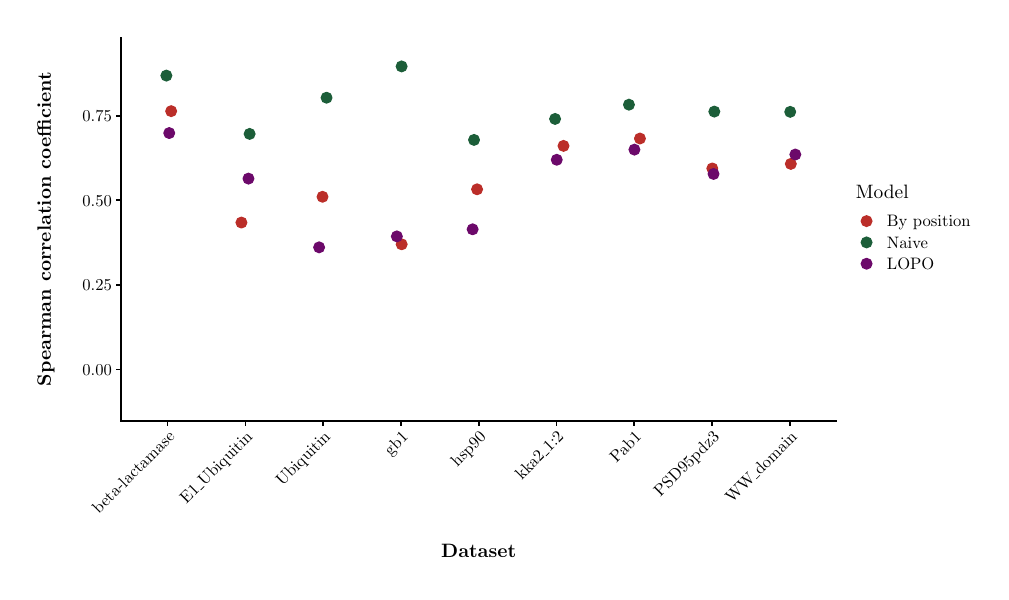
\begin{tikzpicture}[x=1pt,y=1pt]
\definecolor{fillColor}{RGB}{255,255,255}
\path[use as bounding box,fill=fillColor,fill opacity=0.00] (0,0) rectangle (344.26,196.49);
\begin{scope}
\path[clip] ( 33.67, 54.47) rectangle (292.28,192.99);
\definecolor{drawColor}{RGB}{28,94,57}
\definecolor{fillColor}{RGB}{28,94,57}

\path[draw=drawColor,line width= 0.4pt,line join=round,line cap=round,fill=fillColor] ( 80.20,158.10) circle (  1.96);

\path[draw=drawColor,line width= 0.4pt,line join=round,line cap=round,fill=fillColor] (248.12,166.16) circle (  1.96);

\path[draw=drawColor,line width= 0.4pt,line join=round,line cap=round,fill=fillColor] (217.27,168.66) circle (  1.96);

\path[draw=drawColor,line width= 0.4pt,line join=round,line cap=round,fill=fillColor] (108.00,171.18) circle (  1.96);

\path[draw=drawColor,line width= 0.4pt,line join=round,line cap=round,fill=fillColor] (275.54,166.07) circle (  1.96);

\path[draw=drawColor,line width= 0.4pt,line join=round,line cap=round,fill=fillColor] ( 50.12,179.17) circle (  1.96);

\path[draw=drawColor,line width= 0.4pt,line join=round,line cap=round,fill=fillColor] (135.12,182.49) circle (  1.96);

\path[draw=drawColor,line width= 0.4pt,line join=round,line cap=round,fill=fillColor] (161.29,155.93) circle (  1.96);

\path[draw=drawColor,line width= 0.4pt,line join=round,line cap=round,fill=fillColor] (190.58,163.51) circle (  1.96);
\definecolor{drawColor}{RGB}{187,46,41}
\definecolor{fillColor}{RGB}{187,46,41}

\path[draw=drawColor,line width= 0.4pt,line join=round,line cap=round,fill=fillColor] ( 77.24,126.07) circle (  1.96);

\path[draw=drawColor,line width= 0.4pt,line join=round,line cap=round,fill=fillColor] (247.39,145.62) circle (  1.96);

\path[draw=drawColor,line width= 0.4pt,line join=round,line cap=round,fill=fillColor] (221.24,156.43) circle (  1.96);

\path[draw=drawColor,line width= 0.4pt,line join=round,line cap=round,fill=fillColor] (106.54,135.38) circle (  1.96);

\path[draw=drawColor,line width= 0.4pt,line join=round,line cap=round,fill=fillColor] (275.76,147.26) circle (  1.96);

\path[draw=drawColor,line width= 0.4pt,line join=round,line cap=round,fill=fillColor] ( 51.85,166.32) circle (  1.96);

\path[draw=drawColor,line width= 0.4pt,line join=round,line cap=round,fill=fillColor] (135.14,118.21) circle (  1.96);

\path[draw=drawColor,line width= 0.4pt,line join=round,line cap=round,fill=fillColor] (162.39,138.08) circle (  1.96);

\path[draw=drawColor,line width= 0.4pt,line join=round,line cap=round,fill=fillColor] (193.62,153.77) circle (  1.96);
\definecolor{drawColor}{RGB}{108,9,106}
\definecolor{fillColor}{RGB}{108,9,106}

\path[draw=drawColor,line width= 0.4pt,line join=round,line cap=round,fill=fillColor] (191.18,148.75) circle (  1.96);

\path[draw=drawColor,line width= 0.4pt,line join=round,line cap=round,fill=fillColor] (160.78,123.63) circle (  1.96);

\path[draw=drawColor,line width= 0.4pt,line join=round,line cap=round,fill=fillColor] (219.25,152.42) circle (  1.96);

\path[draw=drawColor,line width= 0.4pt,line join=round,line cap=round,fill=fillColor] (133.40,121.07) circle (  1.96);

\path[draw=drawColor,line width= 0.4pt,line join=round,line cap=round,fill=fillColor] (105.31,117.11) circle (  1.96);

\path[draw=drawColor,line width= 0.4pt,line join=round,line cap=round,fill=fillColor] ( 79.78,141.95) circle (  1.96);

\path[draw=drawColor,line width= 0.4pt,line join=round,line cap=round,fill=fillColor] (247.84,143.63) circle (  1.96);

\path[draw=drawColor,line width= 0.4pt,line join=round,line cap=round,fill=fillColor] (277.39,150.65) circle (  1.96);

\path[draw=drawColor,line width= 0.4pt,line join=round,line cap=round,fill=fillColor] ( 51.15,158.41) circle (  1.96);
\end{scope}
\begin{scope}
\path[clip] (  0.00,  0.00) rectangle (344.26,196.49);
\definecolor{drawColor}{RGB}{0,0,0}

\path[draw=drawColor,line width= 0.6pt,line join=round,line cap=rect] ( 33.67, 54.47) --
	( 33.67,192.99);
\end{scope}
\begin{scope}
\path[clip] (  0.00,  0.00) rectangle (344.26,196.49);
\definecolor{drawColor}{RGB}{0,0,0}

\node[text=drawColor,anchor=base east,inner sep=0pt, outer sep=0pt, scale=  0.60] at ( 30.42, 70.93) {0.00};

\node[text=drawColor,anchor=base east,inner sep=0pt, outer sep=0pt, scale=  0.60] at ( 30.42,101.49) {0.25};

\node[text=drawColor,anchor=base east,inner sep=0pt, outer sep=0pt, scale=  0.60] at ( 30.42,132.05) {0.50};

\node[text=drawColor,anchor=base east,inner sep=0pt, outer sep=0pt, scale=  0.60] at ( 30.42,162.62) {0.75};
\end{scope}
\begin{scope}
\path[clip] (  0.00,  0.00) rectangle (344.26,196.49);
\definecolor{drawColor}{RGB}{0,0,0}

\path[draw=drawColor,line width= 0.6pt,line join=round] ( 31.92, 72.99) --
	( 33.67, 72.99);

\path[draw=drawColor,line width= 0.6pt,line join=round] ( 31.92,103.56) --
	( 33.67,103.56);

\path[draw=drawColor,line width= 0.6pt,line join=round] ( 31.92,134.12) --
	( 33.67,134.12);

\path[draw=drawColor,line width= 0.6pt,line join=round] ( 31.92,164.68) --
	( 33.67,164.68);
\end{scope}
\begin{scope}
\path[clip] (  0.00,  0.00) rectangle (344.26,196.49);
\definecolor{drawColor}{RGB}{0,0,0}

\path[draw=drawColor,line width= 0.6pt,line join=round,line cap=rect] ( 33.67, 54.47) --
	(292.28, 54.47);
\end{scope}
\begin{scope}
\path[clip] (  0.00,  0.00) rectangle (344.26,196.49);
\definecolor{drawColor}{RGB}{0,0,0}

\path[draw=drawColor,line width= 0.6pt,line join=round] ( 50.54, 52.72) --
	( 50.54, 54.47);

\path[draw=drawColor,line width= 0.6pt,line join=round] ( 78.65, 52.72) --
	( 78.65, 54.47);

\path[draw=drawColor,line width= 0.6pt,line join=round] (106.76, 52.72) --
	(106.76, 54.47);

\path[draw=drawColor,line width= 0.6pt,line join=round] (134.87, 52.72) --
	(134.87, 54.47);

\path[draw=drawColor,line width= 0.6pt,line join=round] (162.98, 52.72) --
	(162.98, 54.47);

\path[draw=drawColor,line width= 0.6pt,line join=round] (191.09, 52.72) --
	(191.09, 54.47);

\path[draw=drawColor,line width= 0.6pt,line join=round] (219.19, 52.72) --
	(219.19, 54.47);

\path[draw=drawColor,line width= 0.6pt,line join=round] (247.30, 52.72) --
	(247.30, 54.47);

\path[draw=drawColor,line width= 0.6pt,line join=round] (275.41, 52.72) --
	(275.41, 54.47);
\end{scope}
\begin{scope}
\path[clip] (  0.00,  0.00) rectangle (344.26,196.49);
\definecolor{drawColor}{RGB}{0,0,0}

\node[text=drawColor,rotate= 45.00,anchor=base east,inner sep=0pt, outer sep=0pt, scale=  0.60] at ( 53.46, 48.30) {beta-lactamase};

\node[text=drawColor,rotate= 45.00,anchor=base east,inner sep=0pt, outer sep=0pt, scale=  0.60] at ( 81.57, 48.30) {E1\_Ubiquitin};

\node[text=drawColor,rotate= 45.00,anchor=base east,inner sep=0pt, outer sep=0pt, scale=  0.60] at (109.68, 48.30) {Ubiquitin};

\node[text=drawColor,rotate= 45.00,anchor=base east,inner sep=0pt, outer sep=0pt, scale=  0.60] at (137.79, 48.30) {gb1};

\node[text=drawColor,rotate= 45.00,anchor=base east,inner sep=0pt, outer sep=0pt, scale=  0.60] at (165.90, 48.30) {hsp90};

\node[text=drawColor,rotate= 45.00,anchor=base east,inner sep=0pt, outer sep=0pt, scale=  0.60] at (194.01, 48.30) {kka2\_1:2};

\node[text=drawColor,rotate= 45.00,anchor=base east,inner sep=0pt, outer sep=0pt, scale=  0.60] at (222.12, 48.30) {Pab1};

\node[text=drawColor,rotate= 45.00,anchor=base east,inner sep=0pt, outer sep=0pt, scale=  0.60] at (250.23, 48.30) {PSD95pdz3};

\node[text=drawColor,rotate= 45.00,anchor=base east,inner sep=0pt, outer sep=0pt, scale=  0.60] at (278.34, 48.30) {WW\_domain};
\end{scope}
\begin{scope}
\path[clip] (  0.00,  0.00) rectangle (344.26,196.49);
\definecolor{drawColor}{RGB}{0,0,0}

\node[text=drawColor,anchor=base,inner sep=0pt, outer sep=0pt, scale=  0.70] at (162.98,  4.86) {\bfseries Dataset};
\end{scope}
\begin{scope}
\path[clip] (  0.00,  0.00) rectangle (344.26,196.49);
\definecolor{drawColor}{RGB}{0,0,0}

\node[text=drawColor,rotate= 90.00,anchor=base,inner sep=0pt, outer sep=0pt, scale=  0.70] at (  8.39,123.73) {\bfseries Spearman correlation coefficient};
\end{scope}
\begin{scope}
\path[clip] (  0.00,  0.00) rectangle (344.26,196.49);
\definecolor{drawColor}{RGB}{0,0,0}

\node[text=drawColor,anchor=base west,inner sep=0pt, outer sep=0pt, scale=  0.70] at (299.28,134.62) {Model};
\end{scope}
\begin{scope}
\path[clip] (  0.00,  0.00) rectangle (344.26,196.49);
\definecolor{drawColor}{RGB}{187,46,41}
\definecolor{fillColor}{RGB}{187,46,41}

\path[draw=drawColor,line width= 0.4pt,line join=round,line cap=round,fill=fillColor] (303.13,126.59) circle (  1.96);
\end{scope}
\begin{scope}
\path[clip] (  0.00,  0.00) rectangle (344.26,196.49);
\definecolor{drawColor}{RGB}{28,94,57}
\definecolor{fillColor}{RGB}{28,94,57}

\path[draw=drawColor,line width= 0.4pt,line join=round,line cap=round,fill=fillColor] (303.13,118.89) circle (  1.96);
\end{scope}
\begin{scope}
\path[clip] (  0.00,  0.00) rectangle (344.26,196.49);
\definecolor{drawColor}{RGB}{108,9,106}
\definecolor{fillColor}{RGB}{108,9,106}

\path[draw=drawColor,line width= 0.4pt,line join=round,line cap=round,fill=fillColor] (303.13,111.19) circle (  1.96);
\end{scope}
\begin{scope}
\path[clip] (  0.00,  0.00) rectangle (344.26,196.49);
\definecolor{drawColor}{RGB}{0,0,0}

\node[text=drawColor,anchor=base west,inner sep=0pt, outer sep=0pt, scale=  0.60] at (310.48,124.52) {By position};
\end{scope}
\begin{scope}
\path[clip] (  0.00,  0.00) rectangle (344.26,196.49);
\definecolor{drawColor}{RGB}{0,0,0}

\node[text=drawColor,anchor=base west,inner sep=0pt, outer sep=0pt, scale=  0.60] at (310.48,116.82) {Naive};
\end{scope}
\begin{scope}
\path[clip] (  0.00,  0.00) rectangle (344.26,196.49);
\definecolor{drawColor}{RGB}{0,0,0}

\node[text=drawColor,anchor=base west,inner sep=0pt, outer sep=0pt, scale=  0.60] at (310.48,109.12) {LOPO};
\end{scope}
\end{tikzpicture}
